\documentclass[11pt]{oblivoir}
\usepackage[left=2.5cm,right=2.5cm,top=3cm,bottom=3cm,a4paper]{geometry}
\usepackage{hyperref}
\usepackage{amsmath}
\usepackage{indentfirst}
\usepackage{graphicx}
\graphicspath{ {images/} }
\usepackage{float}

\title{Computer Graphics hw4}
\date{2017-05-22}
\author{2014-18992 DongJin Shin}

\begin{document}
	
\maketitle

\section{Recommended Environment}

\begin{itemize}
\item Linux
\item Graphic card supports GLSL $\geq$ 3.3
\item OpenGL $\geq$ 3.0
\item C++ $\geq$ 6.3.1
\item CMake $\geq$ 3.7.2
\end{itemize}

\section{Execution}

\begin{itemize}
\item \verb|mkdir build| (At root directory, where \verb|CMakeLists.txt| is contained)
\item \verb|cd build|
\item \verb|cmake ..|
\item \verb|make|
\item \verb|cd ../hw4/| (Directory should be correct, since it loads \verb|obj| and shader files in relative path)
\item \verb|./hw4|
\end{itemize}

\section{Controls}
\begin{itemize}
\item Arrow keys to move camera position
\item Page Up / Down to dolly in / out
\item Home / End to zoom in / out
\item Mouse drag to rotate
\item Right click to seek
\item ESC to exit
\end{itemize}

\section{Description}
기본적으로 과제에서 주어진 모든 기본 및 추가사항을 구현하였다.
\begin{figure}[H]
  \centering
  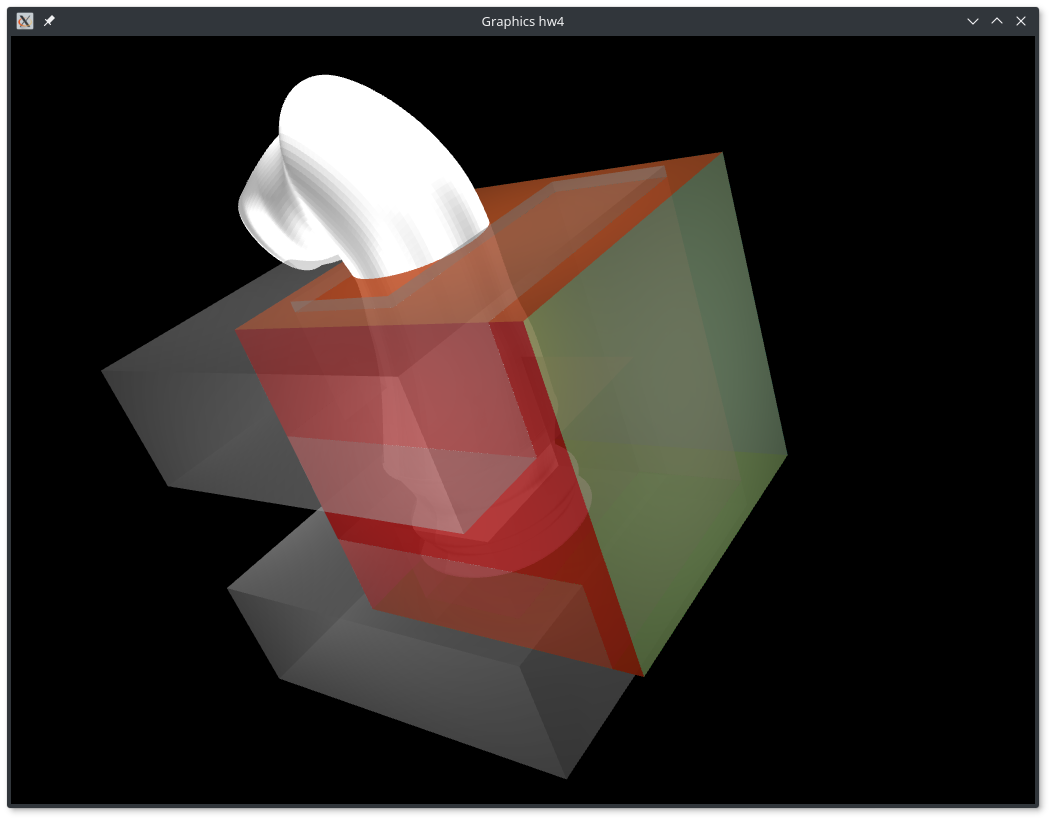
\includegraphics[width=0.75\linewidth]{image1.png}
\end{figure}
\begin{figure}[H]
  \centering
  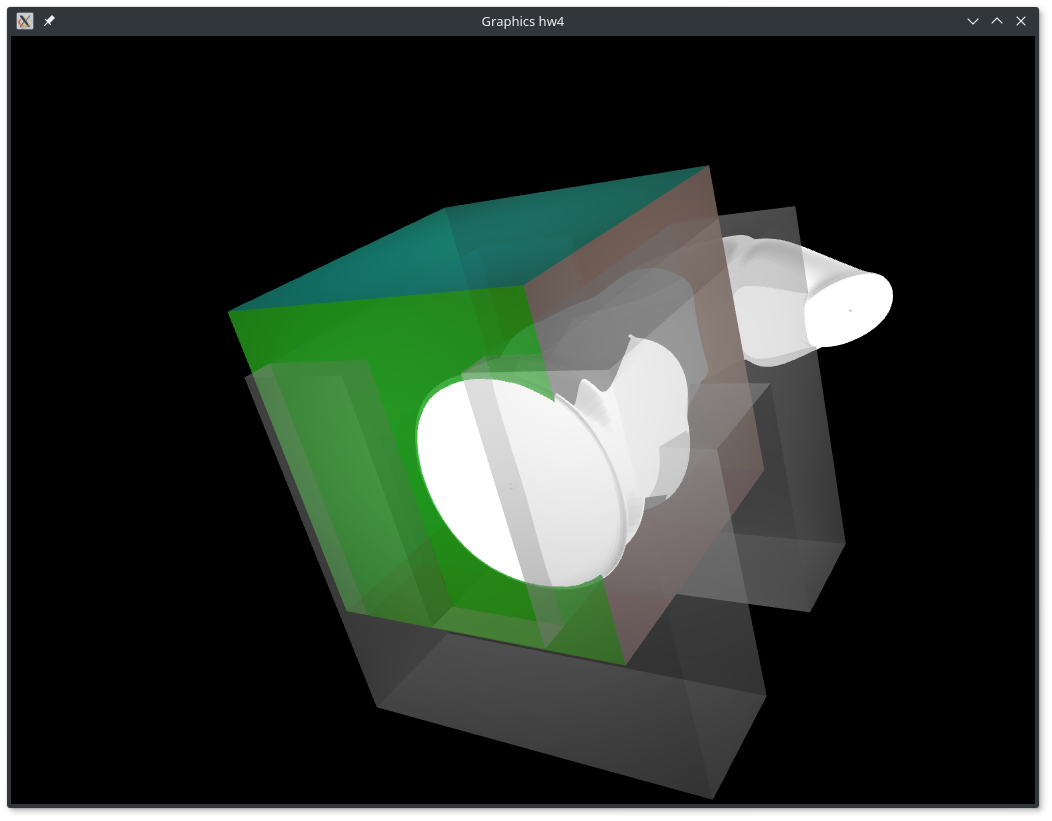
\includegraphics[width=0.75\linewidth]{image2.png}
\end{figure}
\begin{itemize}
\item
  위 이미지로 볼 수 있듯이, 불투명한 체스말, 반투명한 정육면체 그리고 복잡한 반투명 물체로 반투명한 ㄷ자 입체 구조물 총 3개를 겹쳐 shading을 하였다.
\item
  정육면체의 각 면은 서로 다른 ambient, diffuse, specular 계수를 가지게 하여 각각 다른 material을 표현할 수 있도록 구현하였다.

  material에 대한 정보는 \url{http://www.it.hiof.no/~borres/j3d/explain/light/p-materials.html}를 참조하였으며, \verb|main.cpp| 156-185 line에 구현되어 있다.

  각 면의 material은 다음과 같다.
  \begin{itemize}
    \item Yellow Rubber : $K_{a} = (0.05,0.05,0.0)$, $K_{d} = (0.5,0.5,0.4)$, $K_{s} = (0.7,0.7,0.04)$
    \item Chrome : $K_{a} = (0.25, 0.25, 0.25)$, $K_{d} = (0.4,0.4,0.4)$, \\ $K_{s} = (0.774597, 0.774597, 0.774597)$
    \item Copper : $K_{a} = (0.19125, 0.0735, 0.0225)$, $K_{d} = (0.7038, 0.27048, 0.0828)$, $K_{s} = (0.256777, 0.137622, 0.086014)$
    \item Emerald : $K_{a} = (0.0215, 0.1745, 0.0215)$, $K_{d} = (0.07568, 0.61424, 0.07568)$, $K_{s} = (0.633, 0.727811, 0.633)$
    \item Ruby : $K_{a} = (0.1745, 0.01175, 0.01175)$, $K_{d} = (0.61424, 0.04136, 0.04136)$, $K_{s} = (0.727811, 0.626959, 0.626959)$
    \item Cyan Plastic : $K_{a} = (0.0,0.1,0.06)$, $K_{d} = (0.0,0.50980392,0.50980392)$, $K_{s} = (0.50196078,0.50196078,0.50196078)$
  \end{itemize}
\item
  Depth ordering을 위해 BSP tree를 구현하였다. 자세한 구현은 \verb|bsp.h|에서 확인할 수 있다.

  Opaque한 체스말을 가장 먼저 렌더링한 후, 반투명한 표면을 가진 정육면체와 ㄷ자 구조물은 하나의 BSP트리로 구성하여 렌더링 순서를 설정하였다.
\item
  Viewing은 hw2에서부터 구현한 기능을 그대로 사용하였다. Lighting은 총 6개의 백색광을 두어, 정육면체의 각 면 방향에 위치하도록 설정하였다.
  각 광원의 위치는 \verb|main.cpp| 248-253 line에 구현되어 있다.

  모든 광원은 directional light source로 작동하도록 구현하였다.

  효율적인 계산을 위해 셰이더에 6개를 각각 입력하여 연산하였다. 자세한 구현은 \\ \verb|shader/LightShading.frag|에서 확인할 수 있다.

\end{itemize}
\end{document}
